\documentclass[12pt,aspectratio=169]{beamer}

% ====================================================
% ====================================================
% USEPACKAGES AND IMPORTS
% ====================================================
% ====================================================

\usepackage[T1]{fontenc}
\usepackage[utf8]{inputenc}
\usepackage[english]{babel}

% tables
\usepackage{tabularx}
\usepackage{colortbl}
\usepackage{multirow}
\usepackage{makecell}

% tikz and colors
\usepackage{tikz}
\usepackage{xcolor}
\usepackage{pgfplots}
\usepackage{pgfplotstable}
\usepackage{tikzsymbols}

\usetikzlibrary{calc}
\usetikzlibrary{trees}
\usetikzlibrary{patterns}
\usetikzlibrary{shadings}
\usetikzlibrary{positioning}
\usetikzlibrary{intersections}
\usepgfplotslibrary{patchplots}
\usepgfplotslibrary{fillbetween}
\usetikzlibrary{decorations.pathreplacing}

\usetikzlibrary{arrows}
\usetikzlibrary{arrows.meta}

\usetikzlibrary{shapes}
\usetikzlibrary{shapes.arrows}
\usetikzlibrary{shapes.callouts}
\usetikzlibrary{shapes.symbols}
\usetikzlibrary{shapes.geometric}

% boxes
\usepackage[many]{tcolorbox}

% math packages and fonts
\usepackage{bm}
\usepackage{ccfonts}
\usepackage{eulervm}
\usepackage{amsmath}
\usepackage{amsfonts}
\usepackage{amssymb}
\usepackage{amsthm}
\usepackage{mathtools}
\usepackage{nicefrac}
\usepackage{slashed}
\usepackage{bbold}
\usepackage{array}
\usepackage{cancel}

% algorithms and listings
\usepackage[ruled,vlined,linesnumbered]{algorithm2e}
\usepackage{listings}
\usepackage{setspace}

\tcbuselibrary{listings}
\tcbuselibrary{breakable}
\tcbuselibrary{skins}

% misc
\usepackage{soul}
\usepackage{pifont}
\usepackage{skull}
\usepackage{multicol}
\usepackage{animate}
\usepackage{hyperref}
\usepackage{wasysym}
\usepackage[absolute,overlay]{textpos}
\usepackage[hang,flushmargin]{footmisc}

% ====================================================
% ====================================================
% LAYOUT AND THEME
% ====================================================
% ====================================================

\usetheme{Copenhagen}

% color definitions
\definecolor{myblue1}{RGB}{35,119,189}
\definecolor{myblue2}{RGB}{95,179,238}
\definecolor{myblue3}{RGB}{129,168,207}
\definecolor{myblue4}{RGB}{26,89,142}

\definecolor{myred1}{RGB}{247,12,12}

% set theme colors
\setbeamercolor*{structure}{fg=myblue1,bg=blue}
\setbeamercolor*{palette primary}{use=structure,fg=white,bg=structure.fg}
\setbeamercolor*{palette secondary}{use=structure,fg=white,bg=structure.fg!75!black}
\setbeamercolor*{palette tertiary}{use=structure,fg=white,bg=structure.fg!50!black}
\setbeamercolor*{palette quaternary}{fg=black,bg=white}

\setbeamertemplate{itemize item}[circle]
\setbeamertemplate{itemize subitem}[circle]
\setbeamertemplate{itemize subsubitem}[circle]

\setbeamertemplate{enumerate item}[circle]
\setbeamertemplate{enumerate subitem}[circle]
\setbeamertemplate{enumerate subsubitem}[circle]

\setbeamercolor{itemize item}{fg=myblue1}
\setbeamercolor{itemize subitem}{fg=myblue1}
\setbeamercolor{itemize subsubitem}{fg=myblue1}

\setbeamertemplate{section in toc}[circle]
\setbeamertemplate{subsection in toc}[circle]
\setbeamerfont{subsection in toc}{size=\scriptsize}

\setbeamercolor{frametitle continuation}{fg=black}

% title graphic -- sap logo and dhbw logo
\titlegraphic{
\includegraphics[scale=0.1]{../03_img/logo_sap}\hspace*{4.75cm}~%
   	
\includegraphics[scale=0.05]{../03_img/logo_dhbw}
}

\makeatletter
% frame title
\defbeamertemplate*{frametitle}{mydefault}[1][left]
{
  	\ifbeamercolorempty[bg]{frametitle}{}{\nointerlineskip}%
  	\nointerlineskip%
 	\@tempdima=\textwidth%
  	\advance\@tempdima by\beamer@leftmargin%
  	\advance\@tempdima by\beamer@rightmargin%
  	\begin{tcolorbox}[
  		enhanced,
  		outer arc=0pt,
  		arc=0pt,
  		boxrule=0pt,
  		top=0pt,
  		bottom=0pt,
  		enlarge left by=-\beamer@leftmargin,
  		enlarge right by=-\beamer@rightmargin,
  		width=\paperwidth,
  		nobeforeafter,
  		interior style={
    			left color=myblue2,
    			right color=white
    		},
  		shadow={0mm}{-0.4mm}{0mm}{black!60,opacity=0.6},    
  		shadow={0mm}{-0.8mm}{0mm}{black!40,opacity=0.4},    
  	]
    	\usebeamerfont{frametitle}%
    	\vbox{}\vskip-1ex%
    	\if@tempswa\else\csname beamer@fte#1\endcsname\fi%
    	\insertframetitle\par%
    	{%
      		\ifx\insertframesubtitle\@empty%
      		\else%
      		{\usebeamerfont{framesubtitle}\usebeamercolor[fg]{black}\insertframesubtitle\strut\par}%
      		\fi
    	}%
    	\vskip-1ex%
    	\if@tempswa\else\vskip-.3cm\fi
  	\end{tcolorbox}%
}

% footline of a frame
\defbeamertemplate*{footline}{mysplit theme}
{%
  	\leavevmode%
  	\hbox{
		\begin{beamercolorbox}[
			wd=.5\paperwidth,ht=2.5ex,dp=1.125ex,leftskip=.3cm plus1fill,rightskip=.3cm
		]{author in head/foot}%
    			\usebeamerfont{author in head/foot}\insertshortauthor\ (\insertinstitute), \insertdate
  		\end{beamercolorbox}%
  		\begin{beamercolorbox}[
			wd=.5\paperwidth,ht=2.5ex,dp=1.125ex,leftskip=.3cm,rightskip=.3cm plus1fil
		]{title in head/foot}%
    			\usebeamerfont{title in head/foot}\insertshorttitle\hfill
    			\insertprefix-\insertframenumber/\inserttotalframenumber\hspace*{0.5em}
  		\end{beamercolorbox}}%
  	\vskip0pt%
}
\makeatother

% ====================================================
% ====================================================
% COMMANDS AND GENERAL DEFINITIONS
% ====================================================
% ====================================================

% page number prefix
\newcommand\insertprefix{}  % empty by default
\newcommand\prefix[1]{\renewcommand\insertprefix{#1}}

% math definitions
% ====================================================
\DeclareMathOperator*{\argmax}{arg\,max}
\DeclareMathOperator*{\argmin}{arg\,min}
\newcommand*\diff{\mathop{}\!\mathrm{d}}

\newcommand*{\vertbar}{\rule[-1ex]{0.5pt}{2.5ex}}
\newcommand*{\horzbar}{\rule[.5ex]{2.5ex}{0.5pt}}

% commands
% ====================================================

% highlight commands
% --------------------------------------------------------------------------------------------------------
% highlight command
\newcommand{\highlight}[1]{\textcolor{myblue1}{\textbf{#1}}}
\newcommand{\highlighttt}[1]{\textcolor{myblue1}{\texttt{#1}}}
\newcommand{\Highlight}[1]{\textcolor{myred1}{\textbf{#1}}}

% blue color boxes (with frame/without frame/without fill)
\newtcolorbox{boxBlue}{colback=myblue1!10!white,colframe=myblue4}
\newtcolorbox{boxBlueNoFrame}{colback=myblue1!10!white,colframe=myblue1!10!white}
\newtcolorbox{boxBlueNoFill}{colback=white,colframe=myblue4}

% font commands
% --------------------------------------------------------------------------------------------------------
\newcommand{\linkstyle}[1]{\underline{\smash{\texttt{#1}}}} 		% style of hyperlinks

% tikz commands
% --------------------------------------------------------------------------------------------------------

% yellow sticky note
\newcommand{\bubble}[3]{
\begin{textblock}{100}(#1, #2)
      	\begin{tikzpicture}
		\node[rectangle,draw=yellow,very thick,fill=yellow!60,align=center] at (0,0) {#3};
	\end{tikzpicture}
\end{textblock}
}

\newcommand{\floattext}[3]{
\begin{textblock}{100}(#1, #2)
      	#3
\end{textblock}
}

\newcommand{\doublecircle}[2]{
	\draw[fill=white,draw=myblue1] (#1,#2) circle (2mm);
	\draw[fill=myblue1,draw=myblue1] (#1,#2) circle (1.5mm);
}

% slide modifiers
% --------------------------------------------------------------------------------------------------------
% mark slide as optional
\newcommand{\optional}{
	\begin{textblock}{100}(0.15,0.30)
      		
\includegraphics[scale=0.2]{../03_img/scream}
    	\end{textblock}
}

% mark slide as important
\newcommand{\important}{
	\begin{textblock}{100}(0.10,0.15)
      		
\includegraphics[scale=0.1]{../03_img/important}
    	\end{textblock}
}

% citation
% --------------------------------------------------------------------------------------------------------
% first argument in {book, online, article}
\newcommand{\literature}[5]{
	\setbeamertemplate{bibliography item}[#1]
	\bibitem{#2}
	\highlight{#3} \\
	\textcolor{darkgray}{\textit{#4}} \\
	\textcolor{black}{#5}
}
% cite content
\newcommand{\citeAuthor}[3]{\vfill\scriptsize\textcolor{lightgray}{#1 \cite{#2} #3}}

% slide architecture
% --------------------------------------------------------------------------------------------------------
% divide frame into two parts
\newcommand{\divideTwo}[4]{
	\begin{minipage}{#1\textwidth}
		#2
	\end{minipage}
	\hfill
	\begin{minipage}{#3\textwidth}
		#4
	\end{minipage}
}

% divide frame into two parts (start on top)
\newcommand{\divideTwoTop}[4]{
	\begin{minipage}[t]{#1\textwidth}
		#2
	\end{minipage}
	\hfill
	\begin{minipage}[t]{#3\textwidth}
		#4
	\end{minipage}
}

% special pages
% --------------------------------------------------------------------------------------------------------
% title page
\newcommand{\maketitlepage}{
	{
		\beamertemplatenavigationsymbolsempty
		\usebackgroundtemplate{%
			\tikz[overlay,remember picture] \node[opacity=0.2, at=(current page.center)] {
  				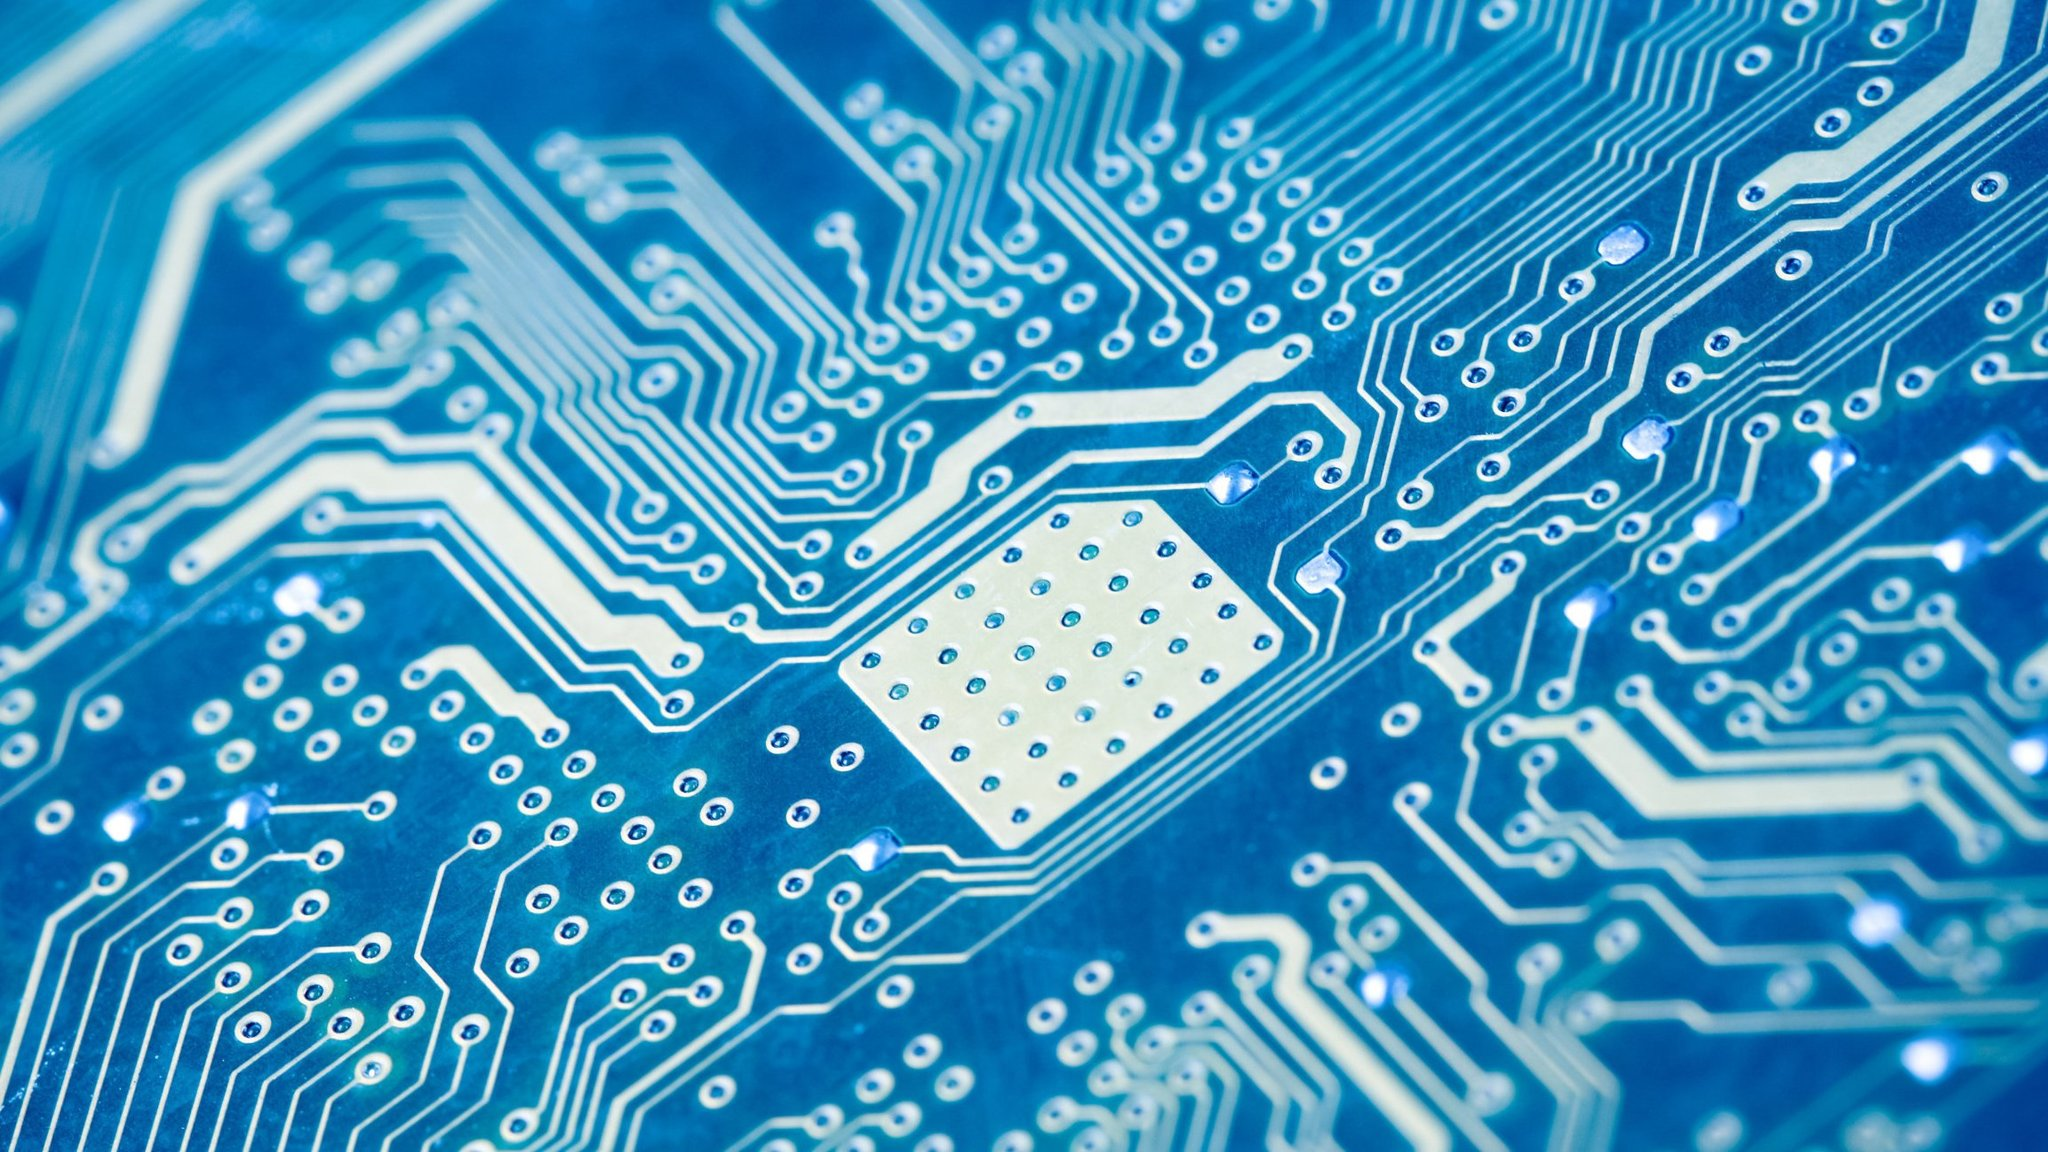
\includegraphics[height=\paperheight,width=\paperwidth]{../03_img/processor.jpg}
			};
		}
		\begin{frame}[plain]
			\vspace*{0.75cm}
			\maketitle
			\vfill
			\begin{center}
				\footnotesize Find all slides on \href{https://github.com/DaWe1992/Applied_ML_Fundamentals}{\linkstyle{GitHub}}
			\end{center}
		\end{frame}
	}
}

% divider page
\newcommand{\makedivider}[1]{
	{
		\beamertemplatenavigationsymbolsempty
		\usebackgroundtemplate{%
			\tikz[overlay,remember picture] \node[opacity=0.2, at=(current page.center)] {
  				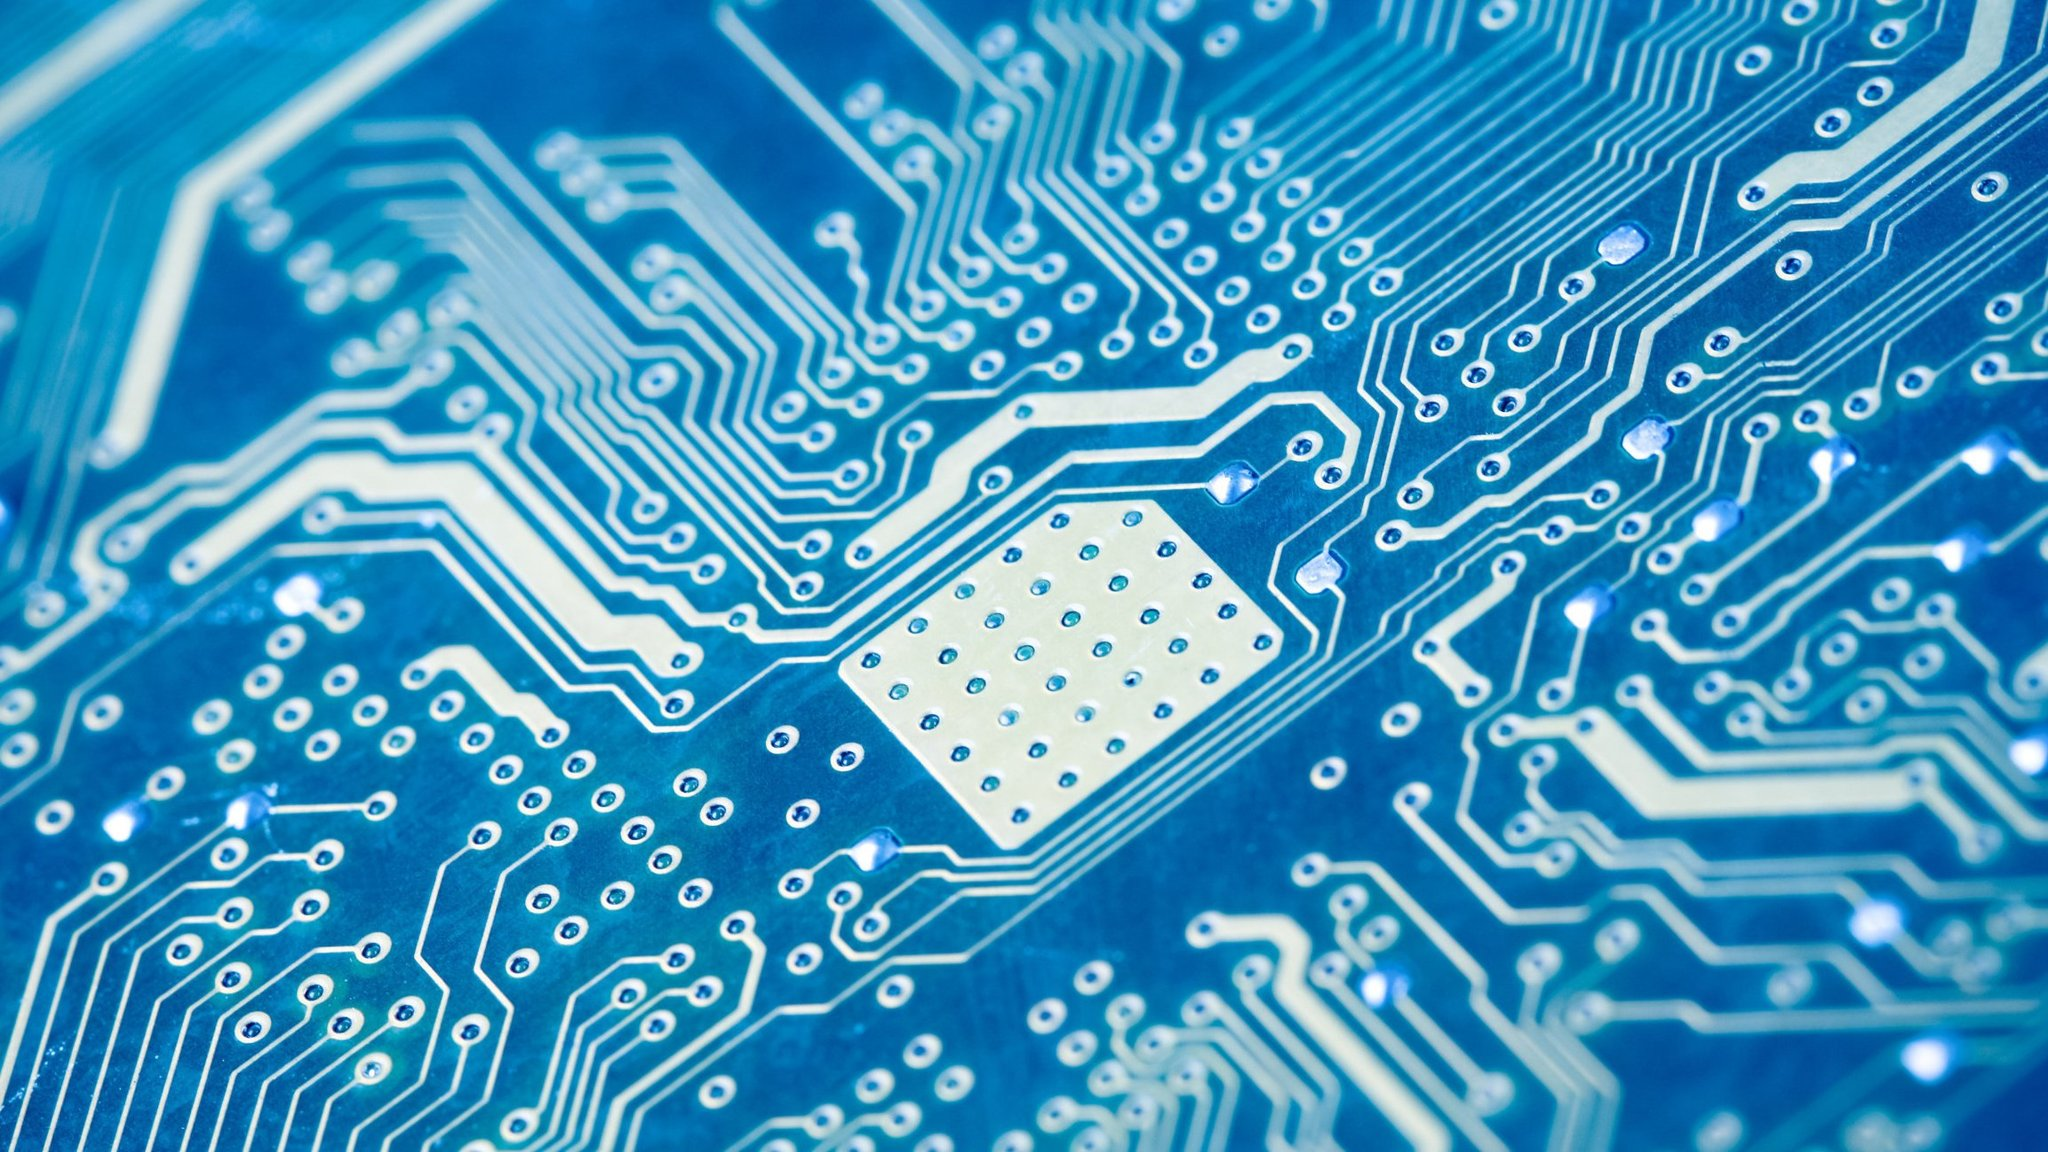
\includegraphics[height=\paperheight,width=\paperwidth]{../03_img/processor.jpg}
			};
		}
		\begin{frame}[plain]
			\vfill
			\begin{boxBlue}
				\centering
				\textbf{Section:} \\
				\large \highlight{#1}
			\end{boxBlue}
			\vfill
			\centering
			
\includegraphics[scale=0.05]{../03_img/logo_dhbw.png}
			\vfill
		\end{frame}
	}
}

% overview page
\newcommand{\makeoverview}[1]{
	\begin{frame}{Lecture Overview}{}
		\begin{tabbing}
			\hspace*{3.5cm}\= \kill
			\ifnum #1=1 \highlight{\textbf{Unit I:}} \else \textbf{Unit I:} \fi
			\> \ifnum #1=1 \highlight{Machine Learning Introduction} \else Machine Learning Introduction \fi \\
		\end{tabbing}
	\end{frame}
}

% thank you page
\newcommand{\makethanks}{
	{\beamertemplatenavigationsymbolsempty
	\begin{frame}[plain]
		\vfill
		\begin{boxBlue}
			\centering
			\Large \highlight{Thank you very much for the attention!}
		\end{boxBlue}
		
		\vfill\footnotesize
		\begin{tabbing}
			\hspace*{1.5cm}\= \kill
			\highlight{Topic:} 	\> \inserttitle \\
			\highlight{Date:} 	\> \insertdate
		\end{tabbing}
		
		\vfill
		\highlight{Contact:} \\
		\insertauthor\ (D062271) \\
		\insertinstitute \\
		\href{mailto:daniel.wehner@sap.com}{\linkstyle{daniel.wehner@sap.com}}
		
		\vfill\normalsize
		\begin{center}
			\large\highlight{Do you have any questions?}
		\end{center}
		\vfill
	\end{frame}}
}

% global pfgplots settings
% --------------------------------------------------------------------------------------------------------
\pgfplotsset{
	% allow filtering of data for pgfplots
	discard if/.style 2 args={
        		x filter/.code={
            		\edef\tempa{\thisrow{#1}}
            		\edef\tempb{#2}
            		\ifx\tempa\tempb
                		\def\pgfmathresult{inf}
            		\fi
        		}
    	},
    	discard if not/.style 2 args={
        		x filter/.code={
            		\edef\tempa{\thisrow{#1}}
            		\edef\tempb{#2}
            		\ifx\tempa\tempb
            		\else
                		\def\pgfmathresult{inf}
            		\fi
        		}
    	}
}


% ====================================================
% ====================================================
% PRESENTATION DATA
% ====================================================
% ====================================================

\title[Principal Component Analysis]{*** Applied Machine Learning Fundamentals *** Principal Component Analysis}
\institute{SAP\,SE}
\author{M.\,Sc. Daniel Wehner}
\date{Winter term 2019/2020}
\prefix{PCA}

% ====================================================
% ====================================================
% BEGIN OF DOCUMENT
% ====================================================
% ====================================================

\begin{document}

% Title frame
%______________________________________________________________________
\maketitlepage


% Lecture Overview
%______________________________________________________________________
\begin{frame}{Lecture Overview}{}
	\makeoverview{10}
\end{frame}


% Agenda
%______________________________________________________________________
\begin{frame}{Agenda for this Unit}
	\begin{multicols}{2}
		\tableofcontents
	\end{multicols}
\end{frame}


% Section: Introduction
%______________________________________________________________________
\section{Introduction}
\makedivider{Introduction}

% Subsection: Why Dimensionality Reduction?
% --------------------------------------------------------------------------------------------------------
\subsection{Why Dimensionality Reduction?}

% Why Dimensionality Reduction?
\begin{frame}{Why Dimensionality Reduction?}{}
	\begin{itemize}
		\item Most data is high-dimensional
		\item Dimensionality reduction can be used for:
		\begin{itemize}
			\item \textbf{Lossy (!)} data compression
			\item Feature extraction
			\item Data visualization
		\end{itemize}
	\end{itemize}
	
	\begin{boxBlueNoFrame}
		Dimensionality reduction can help to \textbf{speed up} learning algorithms substantially.
		Too many (correlated) features usually \textbf{decrease the performance} of the learning algorithm
		(cf. \highlight{curse of dimensionality}).
	\end{boxBlueNoFrame}
\end{frame}


% Subsection: Data Compression
% --------------------------------------------------------------------------------------------------------
\subsection{Data Compression}

% Use Case I: Data Compression / Feature Extraction
\begin{frame}{Use Case I: Data Compression / Feature Extraction}{}
	\divideTwo{0.44}{
		\begin{itemize}
			\item The features \textit{inches} and \textit{cm} are closely related
			\item \textbf{Problems}:
			\begin{itemize}
				\item Redundancy
				\item More memory needed
				\item Algorithms become slow
			\end{itemize}
			\item \textbf{Solution}: Convert $x_1$ and $x_2$ into a new feature $z_1$ \\
				($\mathbb{R}^2 \rightarrow \mathbb{R}$)
		\end{itemize}
	}{0.55}{
		\begin{figure}
	\centering
	\begin{tikzpicture}[
		scale=0.8
	]

		\foreach \x/\y in {0.5/0.8,1/0.75,1.5/1.85,1.75/2,2.35/2.66,3.9/3.45,4.5/4.2}
			\draw[thick] (\x,\y) circle (3pt);

		\draw[very thick,myblue1] (0,0) -- (5,5);

		% axes
		\draw[thick,->] (0,0) -- (5,0) node[right] {$x_1$ (cm)};
		\draw[thick,->] (0,0) -- (0,5) node[left,align=center] {$x_2$\\ (inches)};

		\draw[thick,->] (0,-1) -- (5,-1) node[right] {$z_1$};
		
		\foreach \x in {0.6,0.95,1.55,1.8,2.4,3.7,4.4}
			\draw[thick] (\x,-1) circle (3pt);

	\end{tikzpicture}
\end{figure}
	}
\end{frame}


% Subsection: Data Visualization
% --------------------------------------------------------------------------------------------------------
\subsection{Data Visualization}

% Use Case II: Data Visualization
\begin{frame}{Use Case II: Data Visualization}
	\vspace*{-2mm}
	\divideTwo{0.49}{
		\begin{figure}
			\centering
			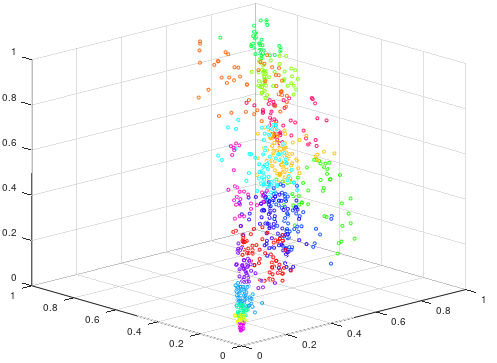
\includegraphics[scale=0.40]{13_pca/02_img/data_viz_3d}
		\end{figure}
	}{0.49}{
		\begin{figure}
			\centering
			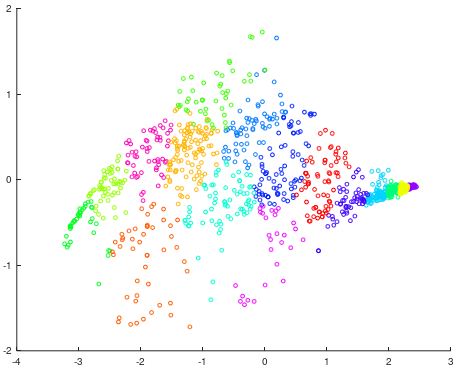
\includegraphics[scale=0.30]{13_pca/02_img/data_viz_2d}
		\end{figure}
	}
\end{frame}


% Subsection: What is PCA?
% --------------------------------------------------------------------------------------------------------
\subsection{What is PCA?}

% PCA: Principal Component Analysis
\begin{frame}{PCA: Principal Component Analysis}{}
	\begin{itemize}
		\item PCA is an \textbf{unsupervised} algorithm
		\item It is known as the \textit{Karhunen-Lo\`{e}ve} transform
		\item PCA can be defined as the \textbf{orthogonal projection} of the data onto a lower dimensional
			\textbf{linear space} (\textit{principal subspace})
		\item Consider a data set of $n$ observations $\bm{X} = \{ \bm{x}^{(1)}, \bm{x}^{(2)}, \dots, \bm{x}^{(n)} \}$
		\begin{itemize}
			\item $\bm{x}^{(i)}$ is a real-valued vector in $\mathbb{R}^m$ ($m$-dimensional)
			\item We want to project the data onto a space having dimensionality $k \ll m$, while \textbf{maximizing
				the variance of the projected data} ($\mathbb{R}^m \rightarrow \mathbb{R}^k$)
		\end{itemize}
		\item \highlight{Remove dimensions which are the least informative of the data}
	\end{itemize}
\end{frame}


% Orthogonal Projections
\begin{frame}{Orthogonal Projections}{}
	\divideTwo{0.66}{
		\begin{figure}
	\centering
	\begin{tikzpicture}[
		scale=0.85
	]

		% axes
		\draw[thick,->] (0,0) -- (9,0) node[right] {$x_1$};
		\draw[thick,->] (0,0) -- (0,5) node[left] {$x_2$};

		\coordinate (L1) at (1,1);
		\coordinate (L2) at (8,4);

		\coordinate (A) at (2,3);
		\coordinate (B) at (3.5,1);
		\coordinate (C) at (4,4.5);
		\coordinate (D) at (7,2.5);

		\coordinate (PA) at ($(L1)!(A)!(L2)$);
		\coordinate (PB) at ($(L1)!(B)!(L2)$);
		\coordinate (PC) at ($(L1)!(C)!(L2)$);
		\coordinate (PD) at ($(L1)!(D)!(L2)$);

		\draw[gray,dashed,thick] (A) -- (PA);
		\draw[gray,dashed,thick] (B) -- (PB);
		\draw[gray,dashed,thick] (C) -- (PC)
			node[below,black] {$\bm{x}_{\perp}^{(i)}$}; \node at (4,5) {$\bm{x}^{(i)}$};
		\draw[gray,dashed,thick] (D) -- (PD);

		\draw[draw=black,fill=gray] (A) circle (4pt);
		\draw[draw=black,fill=gray] (B) circle (4pt);
		\draw[draw=black,fill=gray] (C) circle (4pt);
		\draw[draw=black,fill=gray] (D) circle (4pt);
		
		\draw[very thick,myblue1] (L1) -- (L2);

		\draw[draw=black,fill=myblue1] (PA) circle (4pt);
		\draw[draw=black,fill=myblue1] (PB) circle (4pt);
		\draw[draw=black,fill=myblue1] (PC) circle (4pt);
		\draw[draw=black,fill=myblue1] (PD) circle (4pt);

		\draw[very thick,->] (6.75,4) -- node[above] {$\bm{u}_1$} (7.75,4.429);

	\end{tikzpicture}
\end{figure}
	}{0.33}{
		\begin{itemize}
			\item $\bm{x}^{(i)}$ denote the original data points
			\item $\bm{x}_{\perp}^{(i)}$ is the orthogonal projection of $\bm{x}^{(i)}$ onto vector $\bm{u}_1$ 
		\end{itemize}
	}
\end{frame}


% Section: Maximum Variance Formulation
%______________________________________________________________________
\section{Maximum Variance Formulation}
\makedivider{Maximum Variance Formulation}

% Subsection: Example
% --------------------------------------------------------------------------------------------------------
\subsection{Example}

% Maximum Variance Formulation
\begin{frame}{Maximum Variance Formulation}{}
	\begin{figure}
	\centering
	\begin{tikzpicture}[
		scale=0.75
	]

		% axes
		\draw[thick,->] (-5,0) -- (5,0) node[right] {$x_1$};
		\draw[thick,->] (0,-3.5) -- (0,3.5) node[left,align=center] {$x_2$};

		\coordinate (A) at (-3,-2.25); 	\draw[fill=white] (A) circle (3.5pt);
		\coordinate (B) at (-2,-2); 		\draw[fill=white] (B) circle (3.5pt);
		\coordinate (C) at (1,1); 		\draw[fill=white] (C) circle (3.5pt);
		\coordinate (D) at (2.5,1.8); 	\draw[fill=white] (D) circle (3.5pt);
		\coordinate (E) at (3,2); 		\draw[fill=white] (E) circle (3.5pt);

		\foreach \a/\i in {-0.75/2,-0.5/3,-0.25/4,0/5,0.25/6,0.5/7}{
			\coordinate (L1) at (-4,\a*-4);
			\coordinate (L2) at (4,\a*4);

			\only<\i>\draw[myblue1,very thick] (L1) -- (L2);
			\coordinate (PA) at ($(L1)!(A)!(L2)$);	\only<\i>\draw[red,fill=white] (PA) circle (3.5pt);
			\only<\i>\draw[red,dashed,shorten >=0.1cm,shorten <=0.1cm] (A) -- (PA);
			\coordinate (PB) at ($(L1)!(B)!(L2)$);	\only<\i>\draw[red,fill=white] (PB) circle (3.5pt);
			\only<\i>\draw[red,dashed,shorten >=0.1cm,shorten <=0.1cm] (B) -- (PB);
			\coordinate (PC) at ($(L1)!(C)!(L2)$);	\only<\i>\draw[red,fill=white] (PC) circle (3.5pt);
			\only<\i>\draw[red,dashed,shorten >=0.1cm,shorten <=0.1cm] (C) -- (PC);
			\coordinate (PD) at ($(L1)!(D)!(L2)$);	\only<\i>\draw[red,fill=white] (PD) circle (3.5pt);
			\only<\i>\draw[red,dashed,shorten >=0.1cm,shorten <=0.1cm] (D) -- (PD);
			\coordinate (PE) at ($(L1)!(E)!(L2)$);	\only<\i>\draw[red,fill=white] (PE) circle (3.5pt);
			\only<\i>\draw[red,dashed,shorten >=0.1cm,shorten <=0.1cm] (E) -- (PE);
		}
		
	\end{tikzpicture}
\end{figure}
\end{frame}


% Subsection: Formalization of the Problem
% --------------------------------------------------------------------------------------------------------
\subsection{Formalization of the Problem}

% Maximum Variance Formulation (Ctd.)
\begin{frame}{Maximum Variance Formulation (Ctd.)}{}
	\begin{itemize}
		\item In the following we assume $k = 1$ {\footnotesize (projection onto a line defined by a unit vector $\bm{u}_1$)}
		\item Each data point $\bm{x}^{(i)}$ is projected onto a scalar value $\bm{u}_1^{\intercal} \bm{x}^{(i)}$
		\item The mean of the projected data is $\bm{u}_1^{\intercal} \overline{\bm{x}}$, where $\overline{\bm{x}}$
			is the sample set mean:
		\begin{equation}
			\overline{\bm{x}} = \frac{1}{n} \sum_{i=1}^n \bm{x}^{(i)}
		\end{equation}
		\item The variance of the projected data is given by:
		\begin{equation}
			\frac{1}{n} \sum_{i=1}^n \left( \bm{u}_1^{\intercal} \bm{x}^{(i)} -
				\bm{u}_1^{\intercal} \overline{\bm{x}} \right)^2 = \bm{u}_1^{\intercal} \bm{\Sigma} \bm{u}_1
		\end{equation}
	\end{itemize}
\end{frame}


% Maximum Variance Formulation (Ctd.)
\begin{frame}{Maximum Variance Formulation (Ctd.)}{}\important
	\begin{itemize}
		\vspace*{2mm}
		\item $\bm{\Sigma}$ is the covariance matrix defined by:
		\begin{equation}
			\bm{\Sigma} = \frac{1}{n} \sum_{i = 1}^n \overbracket{
				(\bm{x}^{(i)} - \overline{\bm{x}}) (\bm{x}^{(i)} - \overline{\bm{x}})^{\intercal}
			}^{\text{\textbf{Outer product} $\rightarrow$ \textbf{matrix}}}
		\end{equation}
		\item The projected variance $\bm{u}_1^{\intercal}\bm{\Sigma}\bm{u}_1$ is maximized with respect to $\bm{u}_1$
		\item Constraint: $\Vert \bm{u}_1 \Vert = 1$, otherwise $\bm{u}_1$ grows unboundedly
		\item We have to solve the following optimization problem:
		\begin{equation}
			\max_{\bm{u}_1} \left\{
				\bm{u}_1^{\intercal} \bm{\Sigma} \bm{u}_1 + \lambda_1 (1 - \bm{u}_1^{\intercal} \bm{u}_1)
			\right\}
		\end{equation}
	\end{itemize}
\end{frame}


% Maximum Variance Formulation (Ctd.)
\begin{frame}{Maximum Variance Formulation (Ctd.)}{}\important
	\begin{itemize}
		\item $\nabla_{\bm{u}_1} \{ \bm{u}_1^{\intercal} \bm{\Sigma} \bm{u}_1 +
			\lambda_1 (1 - \bm{u}_1^{\intercal} \bm{u}_1) \} \overset{!}{=} 0
			\qquad\Longrightarrow \bm{\Sigma} \bm{u}_1 = \lambda_1 \bm{u}_1$
		\item This is an \textbf{eigenvalue problem}
		\item The equation tells us that $\bm{u}_1$ must be an eigenvector of $\bm{\Sigma}$
		\item If we left-multiply by $\bm{u}_1^{\intercal}$ and use $\bm{u}_1^{\intercal} \bm{u}_1 = 1$,
			we see: $\bm{u}_1^{\intercal} \bm{\Sigma} \bm{u}_1 = \lambda_1$
	\end{itemize}
	
	\begin{boxBlueNoFrame}
		\highlight{The variance reaches a maximum, if we set $\bm{u}_1$ equal to the eigenvector having the largest
		eigenvalue $\lambda_1$. This eigenvector is the first principal component.}
	\end{boxBlueNoFrame}
\end{frame}


% Maximum Variance Formulation (Ctd.)
\begin{frame}{Maximum Variance Formulation (Ctd.)}{}
	\begin{itemize}
		\item Additional principal components can be defined in an \textbf{incremental fashion}
		\item Choose each new component such that it \textbf{maximizes the remaining projected variance} 
		\item All principal components are \textbf{orthogonal to each other}
		\item Projection onto $k$ dimensions:
		\begin{itemize}
			\item The lower-dimensional space is defined by the $k$ eigenvectors $\bm{u}_1, \bm{u}_2, \dots, \bm{u}_k$ of the
				covariance matrix $\bm{\Sigma}$
			\item These correspond to the $k$ largest eigenvalues $\lambda_1, \lambda_2, \dots, \lambda_k$
		\end{itemize}
	\end{itemize}
\end{frame}


% Section: PCA Algorithm
%______________________________________________________________________
\section{PCA Algorithm}
\makedivider{PCA Algorithm}

% Subsection: The Algorithm
% --------------------------------------------------------------------------------------------------------
\subsection{The Algorithm}

% PCA Algorithm
\begin{frame}[plain]{}{}
	\begin{algorithm}[H]
		\setstretch{1.6}
		\DontPrintSemicolon
		\footnotesize
		\KwIn{Input data $\bm{X} = \{ \bm{x}^{(1)}, \bm{x}^{(2)}, \dots, \bm{x}^{(n)} \} \in \mathbb{R}^{n \times m}$, number of dimensions $k$}
		\KwOut{Projected data $\bm{Z} \in \mathbb{R}^{n \times k}$}
		$\overline{\bm{x}}
			\longleftarrow \frac{1}{n} \sum_{i=1}^n \bm{x}^{(i)}$
			\tcp*[h]{sample set mean}\;
		$\bm{\Sigma}
			\longleftarrow \frac{1}{n} \sum_{i = 1}^n (\bm{x}^{(i)} - \overline{\bm{x}}) (\bm{x}^{(i)}
				- \overline{\bm{x}})^{\intercal}$
				\tcp*[h]{covariance matrix}\;

		Perform \textbf{s}ingular \textbf{v}alue \textbf{d}ecomposition to find the eigenvectors of matrix $\bm{\Sigma}$:
		\begin{equation*}
			[\bm{U}, \bm{S}, \bm{V}] = SVD(\bm{\Sigma})
		\end{equation*}
		\vspace*{-6mm}

		Select first $k$ eigenvectors: $\bm{U}_k \longleftarrow \bm{U}_{(:,:k)}$
			\tcp*[h]{eig.vecs with largest eig.vals.}\;
		$\bm{Z} \longleftarrow \bm{U}_k^{\intercal} \bm{X}$ 
		\caption{PCA Algorithm}
	\end{algorithm}
\end{frame}


% Projection of the Data
\begin{frame}{Projection of the Data}{}
	\begin{itemize}
		\item Matrix $\bm{U}$ is obtained by applying \textbf{singular value decomposition} to $\bm{\Sigma}$
		\begin{equation}
			\bm{U} =
			\begin{bmatrix}
				\vertbar 		& \vertbar 		& 		& \vertbar 			\\
				\bm{u}_1 		& \bm{u}_2 	& \dots 	& \bm{u}_m		\\
				\vertbar 		& \vertbar 		& 		& \vertbar
			\end{bmatrix} \in \mathbb{R}^{m \times m}
		\end{equation}
		\item The projection $\mathbb{R}^m \rightarrow \mathbb{R}^k (k \ll m)$ is performed as follows:
		\begin{equation}
			\begin{bmatrix}
				z_1^{(i)} 	\\
				\vdots 	\\
				z_k^{(i)}
			\end{bmatrix} = 
			\begin{bmatrix}
				\vertbar 		& \vertbar 		& 		& \vertbar 			\\
				\bm{u}_1 		& \bm{u}_2 	& \dots 	& \bm{u}_k		\\
				\vertbar 		& \vertbar 		& 		& \vertbar
			\end{bmatrix}^{\intercal}
			\begin{bmatrix}
				x_1^{(i)} 	\\
				\vdots 	\\
				x_m^{(i)}
			\end{bmatrix}
		\end{equation}
	\end{itemize}
\end{frame}


% Subsection: Example
% --------------------------------------------------------------------------------------------------------
\subsection{Example}

% PCA Result
\begin{frame}{PCA Result}{}
	\vspace*{-1mm}
	\divideTwo{0.49}{
		\begin{figure}
			\centering
			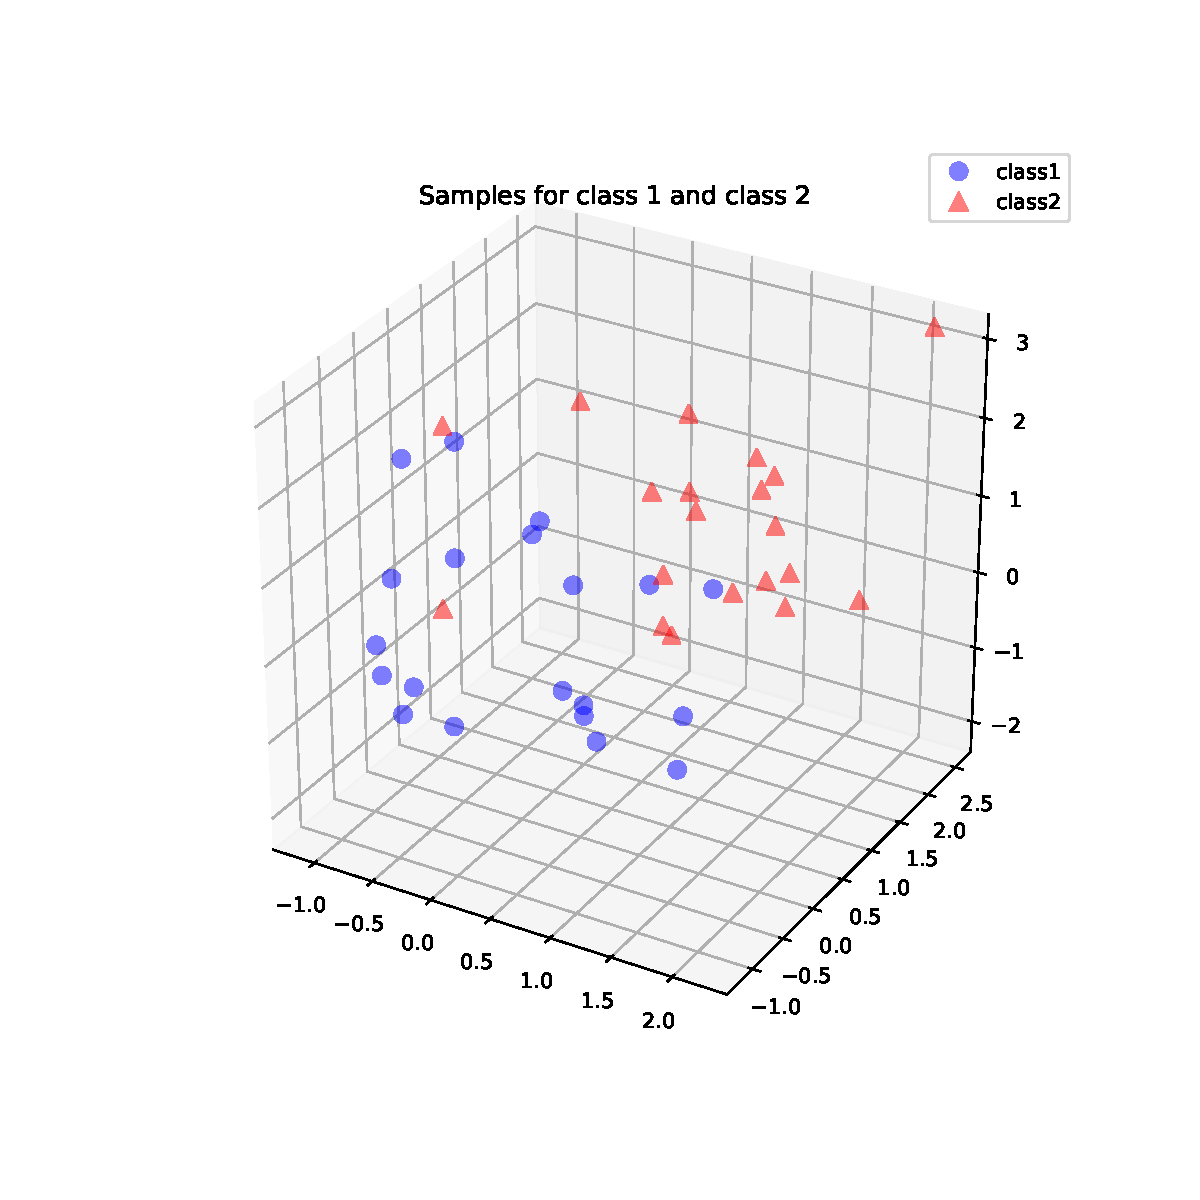
\includegraphics[scale=0.35]{13_pca/02_img/pca_example_data_3d}
		\end{figure}
	}{0.49}{
		\begin{figure}
			\centering
			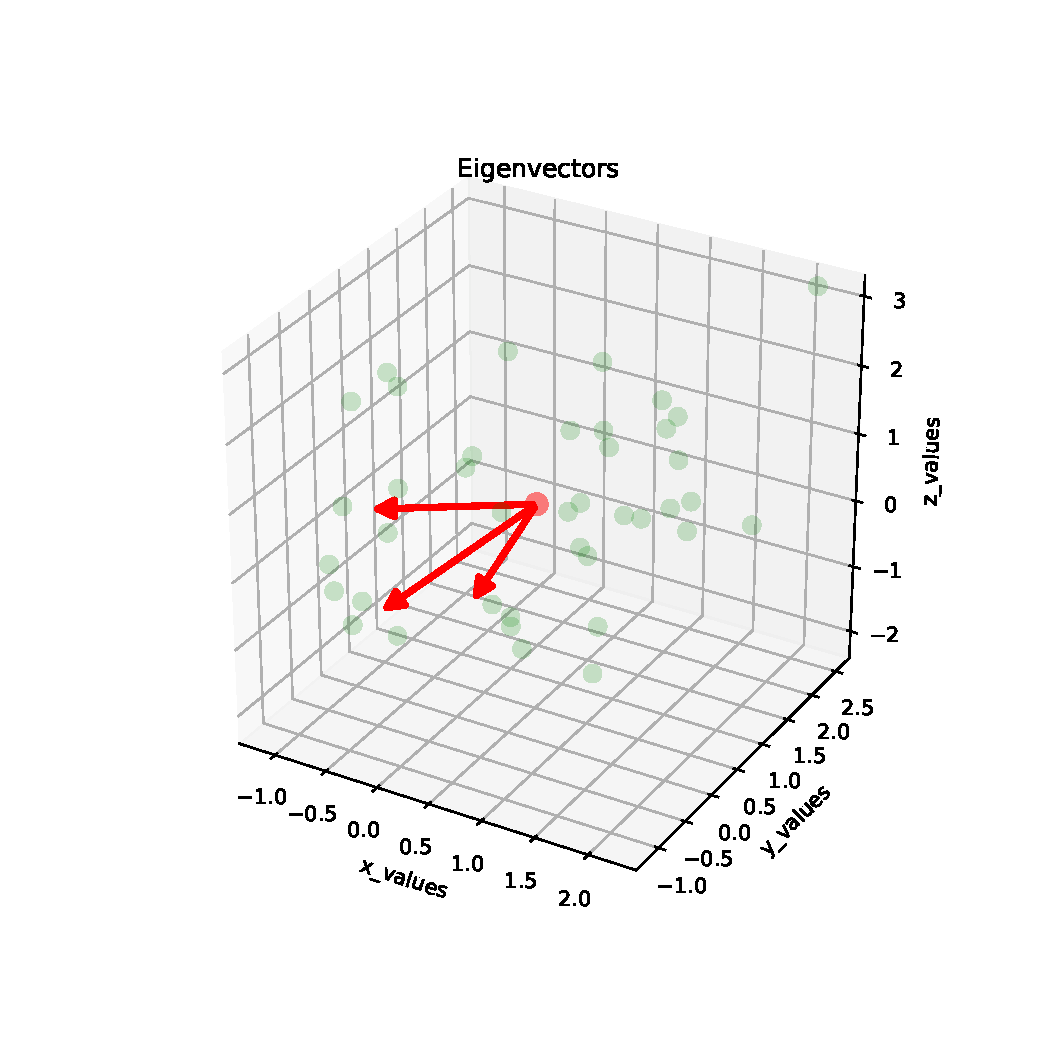
\includegraphics[scale=0.35]{13_pca/02_img/pca_example_eigenvectors}
		\end{figure}
	}
\end{frame}


% PCA Result (Ctd.)
\begin{frame}{PCA Result (Ctd.)}{}
	\begin{figure}
		\centering
		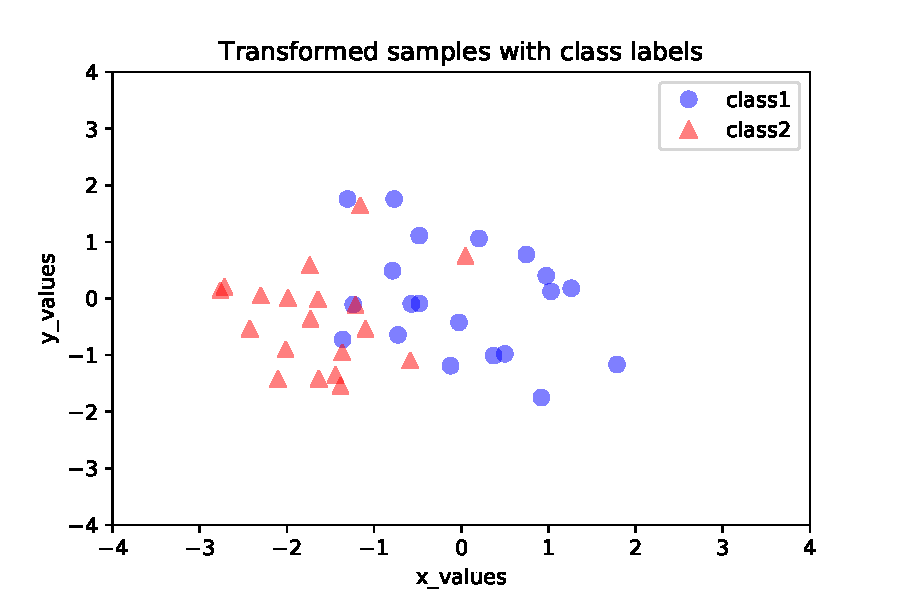
\includegraphics[scale=0.6]{13_pca/02_img/pca_example_data_2d}
	\end{figure}
\end{frame}


% Subsection: Data Reconstruction
% --------------------------------------------------------------------------------------------------------
\subsection{Data Reconstruction}

% Reconstruction from compressed Representation
\begin{frame}{Reconstruction from compressed Representation}{}
	It is possible to compute an approximate reconstruction of the data after having applied PCA ($\mathbb{R}^k \rightarrow \mathbb{R}^m$):
	\begin{equation}
		\bm{x}_{\approx}^{(i)} = \bm{U}_k \bm{z}^{(i)}
	\end{equation}
	\begin{figure}
		\centering
		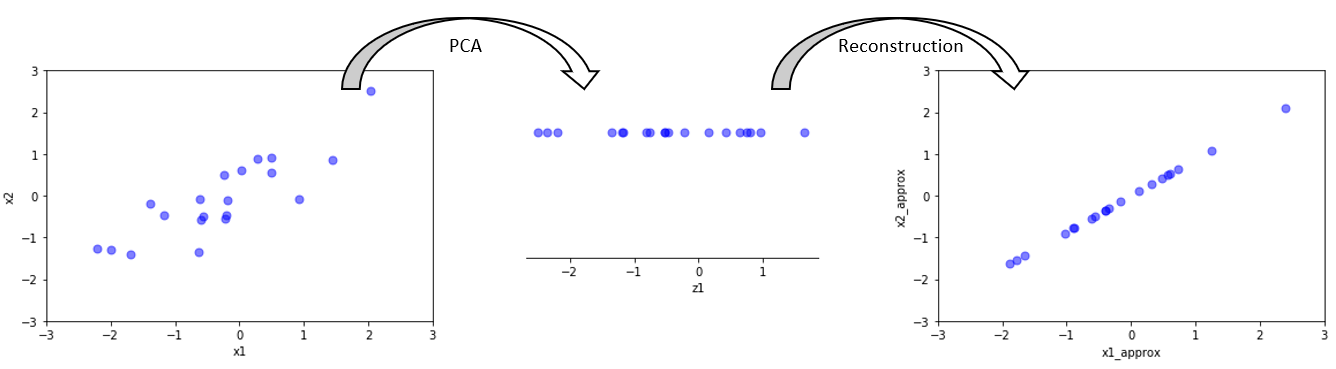
\includegraphics[scale=0.35]{13_pca/02_img/reconstruction}
	\end{figure}
\end{frame}


% Subsection: Choice of $k$
% --------------------------------------------------------------------------------------------------------
\subsection{Choice of $k$}

% Choosing the Number of Components
\begin{frame}{Choosing the Number of Components}{}
	\begin{itemize}
		\item The goal is to preserve as much variance as possible
		\item Minimize the \textbf{average projection error} given by:
		\begin{equation}
			\frac{1}{n} \sum_{i=1}^n \Vert \bm{x}^{(i)} - \bm{x}_{\approx}^{(i)} \Vert^2
		\end{equation}
		\item \textbf{Total variation} in the data is computed as follows:
		\begin{equation}
			\frac{1}{n} \sum_{i=1}^n \Vert \bm{x}^{(i)} \Vert^2
		\end{equation}
	\end{itemize}
\end{frame}


% Choosing the Number of Components (Ctd.)
\begin{frame}{Choosing the Number of Components (Ctd.)}{}
	\begin{itemize}
		\item Typically, $k$ is chosen to be the smallest value such that:
		\begin{equation}
			\frac{
				\overbracket{
					\nicefrac{1}{n} \sum_{i=1}^n \Vert \bm{x}^{(i)} - \bm{x}_{\approx}^{(i)} \Vert^2
				}^{\text{average projection error}}
			}{
				\underbracket{
					\nicefrac{1}{n} \sum_{i=1}^n \Vert \bm{x}^{(i)} \Vert^2
				}_{\text{total variation}}
			} \le \gamma
		\end{equation}
		\item This means that $(1 - \gamma) \cdot 100$\,\% of the variance is retained
	\end{itemize}
\end{frame}


% You can be more efficient...
\begin{frame}{You can be more efficient...}{}
	\begin{itemize}
		\item The above algorithm is computationally very expensive
		\item The same result can be computed much more efficient, remember:
		\begin{equation}
			[\bm{U}, \bm{S}, \bm{V}] = SVD(\bm{\Sigma})
		\end{equation}
		\item We can use the ($m \times m$)-matrix $\bm{S}$ (eigenvalues on the main diagonal):
		\footnotesize
		\begin{equation}
			\bm{S} =
			\begin{bmatrix}
				S_{11} 	& 0 		& \hdots 	& 0 			\\
				0 		& S_{22} 	& \hdots 	& 0 			\\
				\vdots 	& \vdots 	& \ddots 	& \vdots 		\\
				0 		& 0 		& \hdots 	& S_{mm}
			\end{bmatrix}
		\end{equation}
	\end{itemize}
\end{frame}


% You can be more efficient... (Ctd.)
\begin{frame}{You can be more efficient... (Ctd.)}{}\important
	\begin{itemize}
		\item For a given $k$, the fraction of variance retained can be computed as follows:
		\begin{equation}
			1 - \frac{\sum_{i=1}^k S_{ii}}{\sum_{i=1}^m S_{ii}} \le 1 - \gamma
		\end{equation}
		\item The matrix has to be computed only once and can be reused for all $k$
	\end{itemize}
	\begin{boxBlueNoFrame}
		\highlight{Simplification:}
		\begin{equation*}
			\frac{\sum_{i=1}^k S_{ii}}{\sum_{i=1}^m S_{ii}} \ge 1 - \gamma
		\end{equation*}
	\end{boxBlueNoFrame}
\end{frame}


% Section: PCA Applications
%______________________________________________________________________
\section{PCA Applications}
\makedivider{PCA Applications}

% Subsection: Eigenfaces
% --------------------------------------------------------------------------------------------------------
\subsection{Eigenfaces}

% Application of PCA to Images: Eigenfaces
\begin{frame}{Application of PCA to Images: Eigenfaces}{}
	\divideTwo{0.49}{
		\begin{figure}
			\centering
			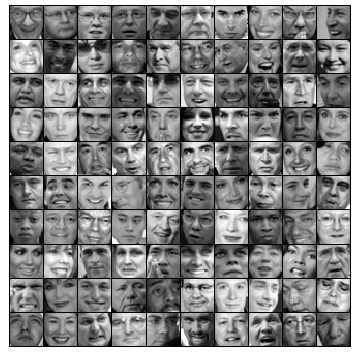
\includegraphics[scale=0.44]{13_pca/02_img/faces}
			\caption{100 images of faces}
		\end{figure}
	}{0.49}{
		\begin{figure}
			\centering
			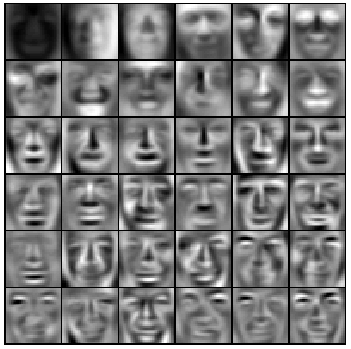
\includegraphics[scale=0.44]{13_pca/02_img/eigenfaces}
			\caption{First 36 principal components}
		\end{figure}
	}
\end{frame}


% Application of PCA to Images: Eigenfaces (Ctd.)
\begin{frame}{Application of PCA to Images: Eigenfaces (Ctd.)}{}
	\divideTwo{0.49}{
		\begin{figure}
			\centering
			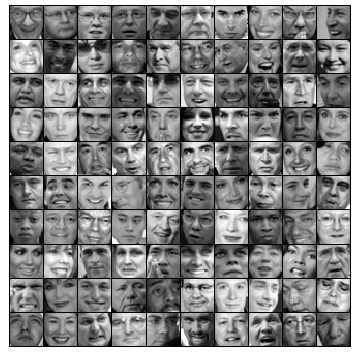
\includegraphics[scale=0.44]{13_pca/02_img/faces}
			\caption{Original images}
		\end{figure}
	}{0.49}{
		\begin{figure}
			\centering
			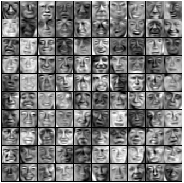
\includegraphics[scale=0.83]{13_pca/02_img/recovered_faces}
			\caption{Reconstructed images}
		\end{figure}
	}
\end{frame}


% Subsection: Face Morphing
% --------------------------------------------------------------------------------------------------------
\subsection{Face Morphing}

% Application of PCA to Images: Face Morphing
\begin{frame}{Application of PCA to Images: Face Morphing}{}
	\begin{figure}
		\centering
		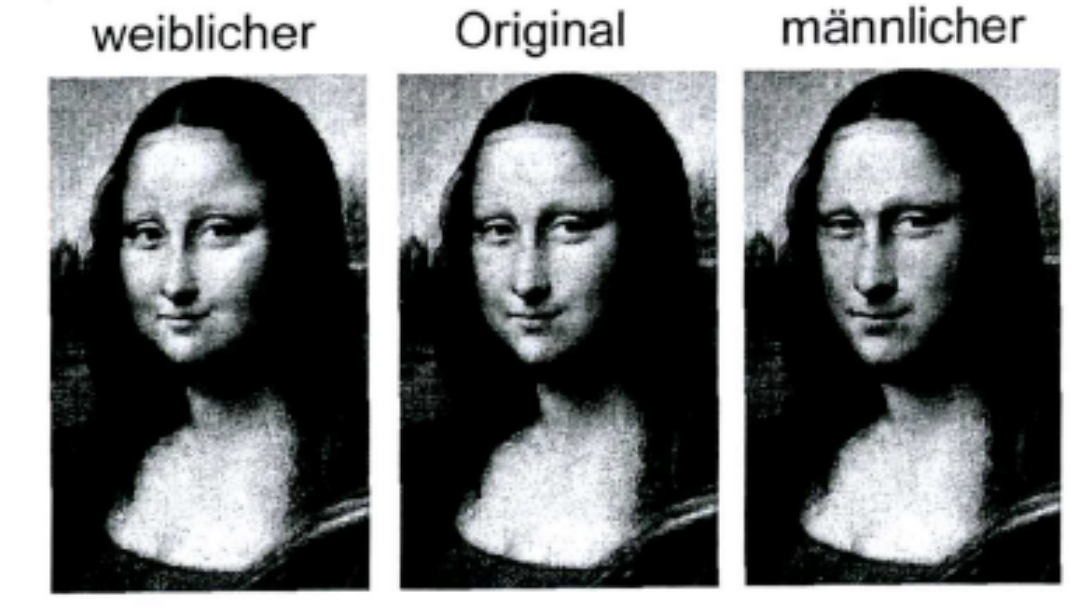
\includegraphics[scale=0.35]{13_pca/02_img/face_morphing}
	\end{figure}
\end{frame}


% Section: Wrap-Up
%______________________________________________________________________
\section{Wrap-Up}
\makedivider{Wrap-Up}

% Subsection: Summary
% --------------------------------------------------------------------------------------------------------
\subsection{Summary}

% Summary
\begin{frame}{Summary}{}
	\begin{itemize}
		\item Dimensionality reduction is important to avoid the \textbf{curse of dimensionality} $\skull$...
		\item ...or simply to \textbf{visualize high-dimensional data}
		\item It is defined as the \textbf{orthogonal projection} of the data onto a lower-dimensional (linear) space
		\item We want to \textbf{keep the dimensions with the most variance}
		\item These dimensions are called \textbf{principal components}
		\item Lots of applications: Eigenfaces, Morphing, ...
	\end{itemize}
\end{frame}


% Subsection: Self-Test Questions
% --------------------------------------------------------------------------------------------------------
\subsection{Self-Test Questions}

% Self-Test Questions
\begin{frame}{Self-Test Questions}{}\important
	\begin{enumerate}
		\item How can PCA be defined?
		\item What is the geometric relationship between the principal components?
		\item Outline the PCA algorithm!
		\item How can you recover the original data? Will you get the exact same data?
		\item Explain how the number of components / dimensions can be chosen!
		\item Name some use cases where PCA is useful!
	\end{enumerate}
\end{frame}


% Subsection: Lecture Outlook
% --------------------------------------------------------------------------------------------------------
\subsection{Lecture Outlook}

\begin{frame}{What's next...?}{}
	\vfill
	\begin{center}
		{\Huge\Highlight{$\skull$ The Exam $\skull$}} \\
		\textit{Just kidding... (maybe)}
	\end{center}
	\vfill
\end{frame}


% Subsection: Recommended Literature and further Reading
% --------------------------------------------------------------------------------------------------------
\subsection{Recommended Literature and further Reading}

% Literature
%______________________________________________________________________
\begin{frame}[allowframebreaks]{Recommended Literature and further Reading}{}
	\footnotesize
	\begin{thebibliography}{2}
		\literature{book}{Bishop.2006}{[1] Pattern Recognition and Machine Learning}
			{Christopher Bishop. Springer. 2006.}{$\rightarrow$ \href{
				http://users.isr.ist.utl.pt/~wurmd/Livros/school/Bishop\%20-\%20Pattern\%20Recognition\%20And\%20Machine\%20Learning\%20-\%20Springer\%20\%202006.pdf
			}{\linkstyle{Link}}, cf. chapter 12.1}
			
		\literature{book}{Murphy.2012}{[2] Machine Learning: A Probabilistic Perspective}
			{Kevin Murphy. MIT Press. 2012.}{$\rightarrow$ \href{
				https://doc.lagout.org/science/Artificial\%20Intelligence/Machine\%20learning/Machine\%20Learning_\%20A\%20Probabilistic\%20Perspective\%20\%5BMurphy\%202012-08-24\%5D.pdf
			}{\linkstyle{Link}}, cf. chapter 12.2}

		\literature{book}{Deisenroth.2019}{[3] Mathematics for Machine Learning}
			{Deisenroth et al. Cambridge University Press. 2019.}{$\rightarrow$ \href{
				https://mml-book.github.io/
			}{\linkstyle{Link}}, cf. chapter 10}
	\end{thebibliography}
\end{frame}


% Subsection: Meme of the Day
% --------------------------------------------------------------------------------------------------------
\subsection{Meme of the Day}

% Meme of the Day
\begin{frame}{Meme of the Day}{}
	\begin{figure}
		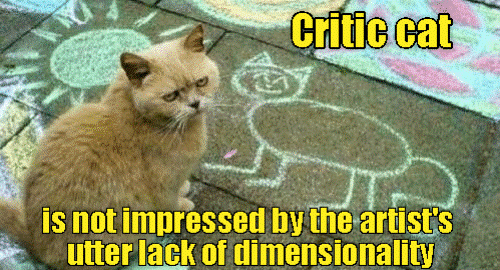
\includegraphics[scale=0.6]{13_pca/02_img/meme_of_the_day}
	\end{figure}
\end{frame}


% Thank you
%______________________________________________________________________
\makethanks

\end{document}